\chapter{CUDA}


CUDA (Compute Unified Device Architecture) është një platformë kompjuterike paralelele dhe model programimi krijuar nga NVIDIA. CUDA është lëshuar në nëntor të vitit 2006 së bashku me kartelën grafike NVIDIA GeForce 8800 GTX, që ishte kartela grafike e parë e ndërtuar me arkitekturën e CUDA-së \cite{cuda_by_example}. Disa muaj pas lansimit të kësaj kartele grafike, NVIDIA bëri publik kompajlerin për këtë gjuhë, CUDA C. CUDA mbështetetet nga këto gjuhë programuese: C, C++, Fortran dhe Python. Kodi mund të ekzekutohet vetëm në pajisjet që posedojnë GPU të NVIDIA. 

\noindent \\ Hapat kryesorë e një programit me CUDA janë: allokimi i memories në GPU, kopjimi i të dhënave nga CPU në GPU, lansimi i kernelit, kopjimi i të dhënave nga GPU në CPU. Ky proces arrihet përmes metodave:	

\begin{itemize}
  \item cudaMalloc – Cuda Memory Allocation. Allokon memorie në GPU. Parametri i parë është pointeri i memoriës të allokuar, kurse parametri i dytë madhësia që duhet të allokohet në bytes. 
  \item 	cudaMemcpy – Cuda Memory Copy. Kopjon të dhëna ndërmjet të CPU dhe GPU. Parametri i parë është adresa e destinacionit të memories, i dyti adresa e burimit të memories, i treti është  madhësia e të dhënave që do të bartim në bytes, dhe i fundit specifikon drejtimin: nëse po kopjojmë nga CPU në GPU ose nga GPU në CPU.
  \item kerneli – metoda që secili thread do e ekzekutojë.
  \item cudaDeviceSynchronize – CPU pret deri sa kernel përfundon ekzekutimin.
\end{itemize}

\noindent Për të demonstruar këto metoda, më poshtë është paraqitur kodi për mbledhjen e dy vargjeve në paralel. \\


\begin{lstlisting}
#include "cuda_runtime.h"
#include "device_launch_parameters.h"

__global__ void addKernel(int *c, int *a, int *b){
    int i = threadIdx.x;
    c[i] = a[i] + b[i];
}

int main(){
    const int arraySize = 5;
    const int a[arraySize] = { 1, 2, 3, 4, 5 };
    const int b[arraySize] = { 10, 20, 30, 40, 50 };
    int c[arraySize] = { 0 };
    
    int* dev_a = 0;
    int* dev_b = 0;
    int* dev_c = 0;
    
    cudaMalloc((void**)&dev_a, arraySize * sizeof(int));
    cudaMalloc((void**)&dev_b, arraySize * sizeof(int));
    cudaMalloc((void**)&dev_c, arraySize * sizeof(int));
    
    cudaMemcpy(dev_a, a, arraySize * sizeof(int), cudaMemcpyHostToDevice);
    cudaMemcpy(dev_b, b, arraySize * sizeof(int), cudaMemcpyHostToDevice);
    
    addKernel << <1, arraySize >> > (dev_c, dev_a, dev_b);
    
    cudaDeviceSynchronize();
    
    cudaMemcpy(c, dev_c, arraySize * sizeof(int), cudaMemcpyDeviceToHost);

    return 0;

}
\end{lstlisting}

\noindent \\Në rreshtin 4 është deklarimi i kernelit. Çdo kernel deklarohet me keywordin \texttt{\_\_global\_\_} dhe nuk duhet të kthejë ndonjë vlerë; prandaj return type e ka \texttt {void}. Metodat tjera që thirren nga kernel, duhet të kenë keywordin \texttt{\_\_device\_\_} dhe mund të kenë return type. Çdo kod që ekzekutohet në GPU quhet device code dhe çdo kod që ekzekutohet në CPU quhet host code.  Në rreshtin 26 është lansimi i kernelit. \texttt{addKernel<<<1,arraySize>>>}  do të thotë se është lansuar kerneli me një bllok me threads sa arraySize. 

\section{CUDA grids, blocks dhe threads}

\noindent Për të organizuar se si threads pasqyrohen në cores në GPU, CUDA ka një hiearki të threadave. Janë 3 levele të kësaj hiearkie; threads, blocks dhe grids. Në nivelin më të ulët të kësaj hiearkie janë threads që i korrespondonjë një CUDA core në GPU kur lansohet kerneli. Një bashkësi threads grupohen në një bllok, dhe blloqet grupohen në një grid. Numri maksimal i threads që mund të i ketë një bllok është 1024.

\noindent \\ Secili grid ka blloqet të organizuara në një dimension 1d, 2d ose 3d. Në figurën \ref{fig:cuda_block_1}, gridi ka strukturë dy dimensionale 3x2, kurse blloku ka strukturë 4x3. Nëse do ta lansonim një kernel me këtë strukturë atëhere në total do të kishim 72 threads që do e ekzekutonin kernelin paralelisht.  Lansimi i këtij kerneli me këtë strukturë do të ishte:\\

\begin{lstlisting}
dim3 grid_size(2, 3, 1);
dim3 block_size(4, 3);
kernel << <grid_size, block_size> >> (...);
\end{lstlisting}

\begin{figure}[!]
    \centering
    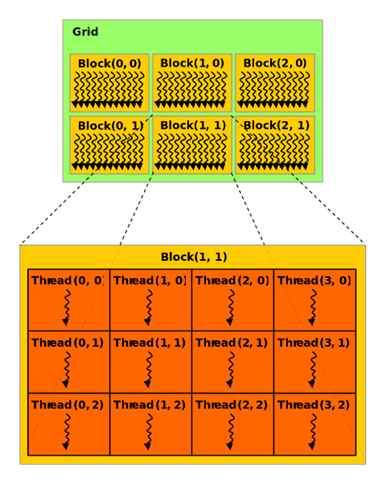
\includegraphics[width=0.45\linewidth]{cuda_1.png}
    \caption{CUDA block me threads \cite{cuda_guide}.}
    \label{fig:cuda_block_1}
\end{figure}


\section{Sinkronizimi i threads}

\noindent Në programim paralel, shpesh nevoitet të i sinkronizojmë threadat, dhe kjo në CUDA arrihet përmes thirrjes së metodës \texttt{\_\_syncthreads()}. Kodi i mëposhtëm ilustron sinkronizimin, ku kemi levizur secilin element të vargut për një në të majtë. Të gjithë threads duhet të mbërrijnë rreshtin 4 para se të vazhdojnë më tutje. Nëse nuk do të sinkronizonim, atëherë do të kishim \textbf{\textit{race-conditions}}, dhe nuk do të kishim fituar rezultatet e pritura. \\


\begin{lstlisting}
__global__ void kernel(int *a){
    int i = threadIdx.x+blockIdx.x*blockDim.x;
    int temp = a[i + 1];
    __synchtreads();
    a[i] = temp;
}
\end{lstlisting}

\noindent \\Sinkronizimi \texttt{\_\_syncthreads()} ndodh vetëm mes threadave të bllokut. Pra nësë do kishim lansuar dy blloqe të threadave, threads të bllokut të dytë nuk do të prisnin threads të bllokut të parë për sinkronizim. Gjatë përpunimit të fraktaleve, nevoitet që të gjithë threads të sinkronizohen mes vete, pra nevoitet sinkronizim edhe mes blloqeve, dhe kjo mund të arrihet duke shfrytëzuar grupet kooperative nga CUDA \cite{cuda_guide}.

\noindent \\ Kodi më poshtëm paraqet një lansim të kernelit që do të shfrytëzojë sinkronizimin mes blloqeve. Në rreshtat 16-20 shikojmë se a i suporton kartela jonë grafike grupet kooperative. Kur do përdorim grupet koperative, duhet të përdorim secilin thread në GPU, dhe do të kemi shfrytëzim 100\% të GPU. Metoda në rreshtin e 24 gjen se me sa threads dhe sa blloqe duhet ta lansojmë kernelin. Pra, nuk kemi mundësi që të lansojmë blloqe ose threads sipas dëshirës sonë. Në rreshtat 27 dhe 28 vërejmë se kemi një lansim tjetër të kernelit. Të gjitha pointerat që do i ketë  kerneli do i ruajmë në një varg, dhe në rreshtin e 28 e bëjmë lansimin e kernelit sipas metodës të dhënë. \\

\begin{lstlisting}
#include "cuda_runtime.h"
#include "device_launch_parameters.h"
#include <cuda_runtime.h>
#include <cooperative_groups.h>

using namespace std;
using namespace cooperative_groups;
namespace cg = cooperative_groups;

__global__ void kernel() {
    auto g = cg::this_grid();
    //Kernel Code
    g.sync();
}

int main() {
    int dev = 0;
    int supportsCoopLaunch = 0;
    cudaDeviceGetAttribute(&supportsCoopLaunch, cudaDevAttrCooperativeLaunch, dev);
    printf("Does this GPU support cooperative Launch?: ", supportsCoopLaunch);

    int threads;
    int blocks;
    cudaOccupancyMaxPotentialBlockSize(&blocks, &threads, kernel, 0, 0);

    //Kernel Launch
    void* kernelArgs[] = { nullptr };
    cudaLaunchCooperativeKernel((void*)kernel, blocks, threads, kernelArgs,0,0);
    return 0;
}

\end{lstlisting}

\section{CUDA-OpenGL interop}
\noindent OpenGL (Open Graphics Library) është një API e përdorur për paraqitjen e grafikave 2D dhe 3D. OpenGl mundëson grafika me perfomancë të lartë duke bashkëvepruar me GPU dhe shfrytëzohet për video-lojëra, programet CAD, realitetin virtual dhe vizualizime shkencore \cite{opengl}.

\noindent \\ Në hyrje të këtij kapitulli, ne kuptuam se kur përpunojmë llogaritje në paralel, kemi bartje të të dhënave nga CPU në GPU, dhe anasjelltas. Bartja e të dhënave merr kohë, dhe nuk është efikase që për secilin frame të ri të bëjmë këso lloj bartjesh. Prandaj ekziston mundësia  që llogaritjet e bëra në GPU, të mos tranferohen në CPU, por të lexohen direkt në GPU nga OpenGL, dhe kjo veti nihet si interoperobaliteti i CUDA dhe OpenGL \cite{cuda_guide}. 

\noindent \\ Kodi i mëposhtëm paraqet se si bëjmë ndërlidhjen e CUDA me OpenGL \cite{cuda_by_example}. Procesi fillon duke i treguar OpenGL se me cilën GPU do të punojë(5-14).  Në rreshtat 20-22 kemi gjeneruar një buffer të OpenGL për të ruajtje të kulmeve(pikave) për një figurë. Ky buffer ndodhet në memorien e GPU dhe menaxhohet nga OpenGL.  Në rreshtin 24 kemi lejuar që  CUDA të ketë qasje në këtë regjister për shkrim dhe lexim të të dhënave.\\

\begin{lstlisting}
GLuint bufferObj;
cudaGraphicsResource* resource;
void setUpCudaOpenGLInterop() {
    //Choose the most suitable CUDA device based on the specified properties(in prop) for openGL.
    cudaDeviceProp prop;
    int dev;
    memset(&prop, 0, sizeof(cudaDeviceProp));
    prop.major = 1;
    prop.minor = 0;
    cudaError_t error = cudaChooseDevice(&dev, &prop);
    if (error != cudaSuccess) {
        printf("Error choosing CUDA device: %s\n", cudaGetErrorString(error));
    }
    cudaGLSetGLDevice(dev);
    //Buffer Size
    iterations = 10;
    numVertices = numberOfVertices(25);
    size_t bufferSize = 2 * numVertices * sizeof(float); //each point has 2 components x,y 
    //Generate openGL buffer
    glGenBuffers(1, &bufferObj);
    glBindBuffer(GL_ARRAY_BUFFER, bufferObj); //Set the context of this buffer obj. In our case its a vertex obj buffer
    glBufferData(GL_ARRAY_BUFFER, bufferSize, NULL, GL_DYNAMIC_COPY); 
    //Notify CUDA runtime that we intend to share the OpenGL buffer named bufferObj with CUDA.
    cudaGraphicsGLRegisterBuffer(&resource, bufferObj, cudaGraphicsMapFlagsNone);
}

\end{lstlisting}

\noindent \\ Tani marrim pointerin e  kulmeve (pikave) të figurës në GPU, dhe këtë pointer ia dergojmë kernelit i cili do e mbush këtë varg me kordinata të pikave. Pas përfundimit të ekzekutimit të kernelit,  njoftojmë OpenGL se CUDA ka përfunduar llogaritjet dhe se vargu i pikave mund të qaset sërish nga OpenGL.\\

\begin{lstlisting}
float* devPtr;
size_t size;
cudaGraphicsMapResources(1, &resource, NULL);
cudaGraphicsResourceGetMappedPointer((void**)&devPtr, &size, resource);
kernel << <blocks, threads >> > (devPtr,..)
cudaGraphicsUnmapResources(1, &resource, NULL);
\end{lstlisting}

\noindent \\ Hapi i fundit është vizualisimi i këtyre pikave. Kodi më poshtë lidh pikat me vijë , me ngjyrë dhe madhësi të caktuar. \\
\begin{lstlisting}
glColor3f(0.29f, 0.44f, 0.55f);
glPointSize(7.0f);
glVertexAttribPointer(0, 2, GL_FLOAT, GL_FALSE, 0, nullptr);
glEnableVertexAttribArray(0);
glDrawArrays(GL_LINE_LOOP, 0, numberOfPoints);
\end{lstlisting}


